\section{Light} \index{Light! Form III topic}

\begin{multicols}{2}


\section*{Reflection from Curved \hfill \\ Surfaces} \index{Mirrors! curved}


\subsection[Radius of Curvature of a Concave Mirror]{Radius of Curvature of a \hfill \\ Concave Mirror}

\begin{center}
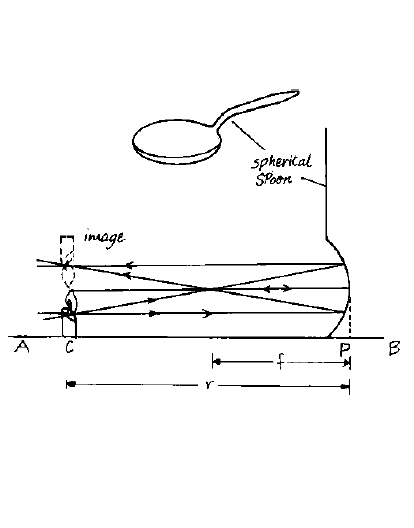
\includegraphics[width=0.49\textwidth]{./img/source/radius-concave.png}
\end{center}

\begin{description*}
%\item[Subtopic:]{}
\item[Materials:]{Spoon, candle/pin, paper}
\item[Setup:]{Draw a line AB on a sheet of paper. Place a concave mirror (spoon) on the paper with its centre vertically above P. Place a lit candle in front of the mirror on line AB as shown.}
\item[Procedure:]{Move the candle along line AB to get a point C where the inverted image of the candle coincides with the object candle.}
%\item[Hazards:]{}
\item[Questions:]{Measure the radius of curvature CP = $r$. Compare the values of $f$ and $r$. Draw ray diagrams to show how the mirror forms images of objects at different positions.}
%\item[Observations:]{}
\item[Theory:]{From the ray diagram, C is the centre of curvature and so $r=2f$. Ray diagrams show that the \emph{concave mirror} produces a real, inverted and magnified image when the object is beyond F. If the object is closer than F, the image appears behind the mirror (virtual), is erect and magnified.}
\item[Applications:]{Shaving mirror, dentist's mirror, floodlight, torch, car headlight}
\item[Notes:]{The mirror works best as a shaving mirror when the object is closer than F.}
\end{description*}

\vfill
\columnbreak

\subsection{Concave and Convex Analogy}

\begin{center}
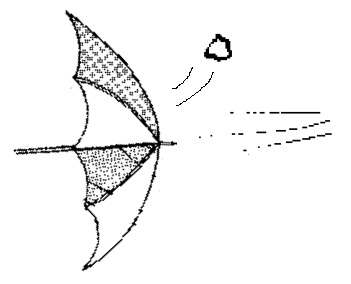
\includegraphics[width=0.3\textwidth]{./img/source/umbrella.png}
\end{center}

\begin{description*}
%\item[Subtopic:]{}
\item[Materials:]{Umbrella, paper}
%\item[Setup:]{}
\item[Procedure:]{One person holds an umbrella horizontally and another throws a crumpled up piece of paper at it. Try to hit above and below the center. Repeat for the inside of the umbrella.}
%\item[Hazards:]{}
%\item[Questions:]{}
\item[Observations:]{The paper balls bounce off the umbrella radially outward for the outer surface, and radially inward off of the inner surface.}
\item[Theory:]{The paper balls represent rays of light which strike the surface of the curved umbrella (mirror) and reflect radially from the focus of the curved surface. The outer surface of the umbrella represents a convex mirror; the inner surface a concave mirror.}
%\item[Applications:]{}
\item[Notes:]{Be sure to throw the paper balls as horizontally as possible.}
\end{description*}

%\subsection{Focus of a Concave Mirror}
%
%\begin{center}
%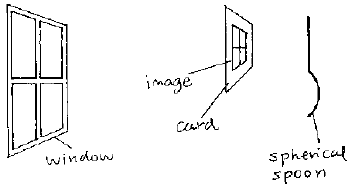
\includegraphics[width=0.4\textwidth]{./img/source/focus-concave.png}
%\end{center}
%
%\begin{description*}
%%\item[Subtopic:]{}
%\item[Materials:]{Spoon, white card}
%%\item[Setup:]{}
%\item[Procedure:]{Hold a white card in front of a curved mirror (spoon) as shown. Point it towards a distant window so that the image of the window can be seen on the card. Move the spoon so that it gives a clear image.}
%%\item[Hazards:]{}
%%\item[Questions:]{Draw the ray diagram for this experiment.}
%\item[Observations:]{The distance from the mirror to the card is known as the \emph{image distance}.}
%\item[Theory:]{Since the window is distant, its rays meet the mirror parallel and hence are reflected through the focus, F. Thus the image distance recorded gives $f$, the focal length of the mirror.}
%%\item[Applications:]{}
%%\item[Notes:]{}
%\end{description*}

\subsection{Images in a Convex Mirror}

\begin{center}
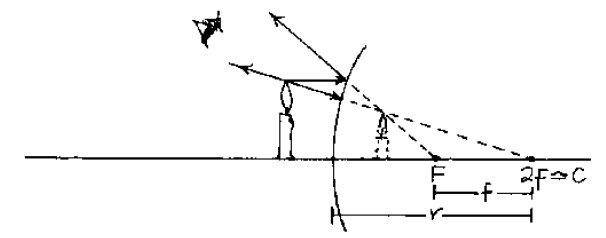
\includegraphics[width=0.42\textwidth]{./img/source/images-convex.png}
\end{center}

\begin{description*}
%\item[Subtopic:]{}
\item[Materials:]{Spoon, candle/pin, paper}
%\item[Setup:]{}
\item[Procedure:]{Arrange a convex mirror (spoon) and lit candle on a piece of paper as shown. Locate the image formed using a pin or lit candle behind the mirror.}
%\item[Hazards:]{}
\item[Questions:]{Mark the position of the object, mirror and image. Measure the object size, object distance and image distance. Draw the ray diagram to show how the convex mirror forms images.}
%\item[Observations:]{}
\item[Theory:]{The image seen is always virtual, erect and reduced in size.}
\item[Applications:]{Rearview mirror in cars, supermarket surveillance}
%\item[Notes:]{Convex mirrors are beneficial for giving a broad field of view.}
\end{description*}

%\subsection{Solar Cooker}
%
%\begin{center}
%\includegraphics[width=0.4\textwidth]{./img/source/.png}
%\end{center}
%
%\begin{description*}
%%\item[Subtopic:]{}
%\item[Materials:]{}
%\item[Setup:]{}
%\item[Procedure:]{}
%\item[Hazards:]{}
%\item[Questions:]{}
%\item[Observations:]{}
%\item[Theory:]{}
%\item[Applications:]{}
%\item[Notes:]{}
%\end{description*}

%==================================================================================================%

\section*{Refraction through Plane \hfill \\ Media} \index{Refraction}


\subsection{Rising Coin}

\begin{center}
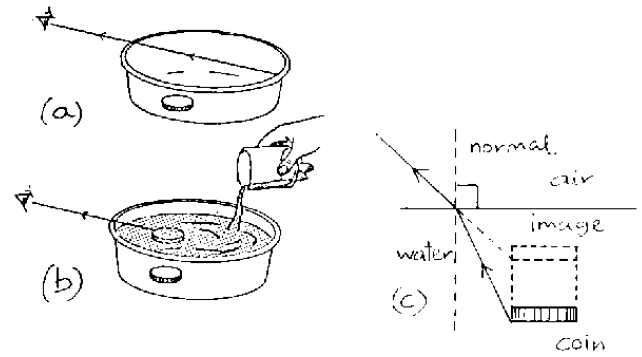
\includegraphics[width=0.49\textwidth]{./img/source/rising-coin.png}
\end{center}

\begin{description*}
%\item[Subtopic:]{}
\item[Materials:]{Coin, dish of water}
%\item[Setup:]{}
\item[Procedure:]{Put a coin in a dish of water. Look across the edge of the lid so the coin is just not visible. Ask someone to gently pour water into the dish, so the eye does not change position.}
%\item[Hazards:]{}
\item[Questions:]{What do you see after adding water?}
\item[Observations:]{The coin becomes visible and appears to have risen in the water.}
\item[Theory:]{The ray diagram in (c) shows that we can only see the coin because the light rays coming from it are \emph{refracted} at the water surface away from the normal of the water surface.}
%\item[Applications:]{}
%\item[Notes:]{}
\end{description*}

\subsection{Bending a Pencil with Water}

\begin{center}
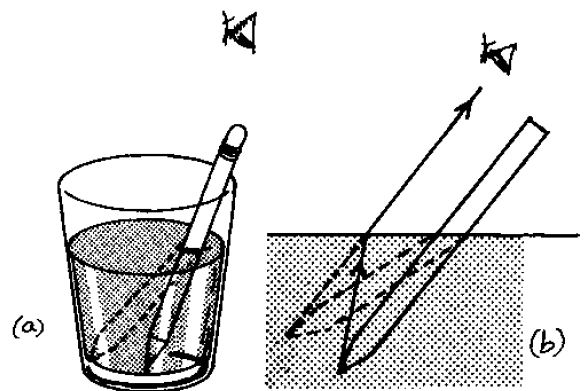
\includegraphics[width=0.45\textwidth]{./img/source/bending-pencil.png}
\end{center}

\begin{description*}
%\item[Subtopic:]{}
\item[Materials:]{Glass, pencil, water}
%\item[Setup:]{}
\item[Procedure:]{Pour water in a glass. Place a pencil in the water at a slant (a). Look at the pencil through the surface of the water from the side along its length and note what you see.}
%\item[Hazards:]{}
%\item[Questions:]{}
\item[Observations:]{The pencil seems to be bent.}
\item[Theory:]{The ray diagram in (b) explains the observation. Light from the tip of the pencil is refracted at the surface of the water and appears to the eye to be bent.}
%\item[Applications:]{}
%\item[Notes:]{}
\end{description*}

\subsection{Candle in Water}

\begin{center}
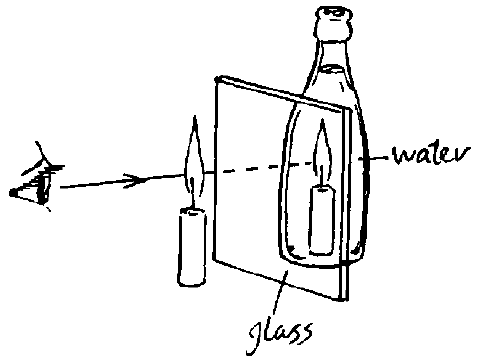
\includegraphics[width=0.42\textwidth]{./img/source/candle-in-water.png}
\end{center}

\begin{description*}
%\item[Subtopic:]{}
\item[Materials:]{Glass plane, bottle of water, candle}
%\item[Setup:]{}
\item[Procedure:]{Place a transparent glass plane midway between a lit candle and a bottle full of water. View the bottle through the glass plane from the side of the candle.}
%\item[Hazards:]{}
%\item[Questions:]{}
\item[Observations:]{The candle appears to burn in the water in the bottle.}
\item[Theory:]{The light from the candle is refracted by the glass plane, causing it to appear within the bottle.}
%\item[Applications:]{}
%\item[Notes:]{}
\end{description*}

\subsection{Refractive Index of Water} \index{Refraction! in water} \index{Practicals! refractive index}
\textbf{*NECTA PRACTICAL*}

\begin{center}
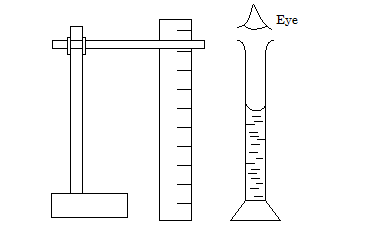
\includegraphics[width=0.45\textwidth]{./img/refractive-index-water.png}
\end{center}

\begin{description*}
%\item[Subtopic:]{}
\item[Materials:]{\nameref{sec:meascyl}, \nameref{sec:retort-stand}, metre rule, pins}
\item[Setup:]{Pour 150 mL of water into the measuring cylinder and drop a pin to the bottom. Look in the measuring cylinder from above. Move another pin up and down outside the cylinder to locate the image position by the no parallax method. Record the depth of the image ($H_1$) and of the water ($H_2$). Repeat for 175 mL, 200 mL, 225 mL and 250 mL.}
%\item[Procedure:]{}
%\item[Hazards:]{}
\item[Questions:]{Plot a graph of $H_2$ (vertical axis) against $H_1$ (horizontal axis). Find the slope and give its physical meaning.}
%\item[Observations:]{}
\item[Theory:]{$H_1$ is the \emph{apparent depth} of the pin, while $H_2$ is the \emph{actual depth}. Refractive index, $\eta$, is found by $\eta = \frac{\text{real depth}}{\text{apparent depth}}$, so the slope of the graph gives the refractive index of water, which should be around 1.33.}
%\item[Applications:]{}
%\item[Notes:]{}
\end{description*}

\subsection{Refractive Index of Glass} \label{sub:refr-index-glass} \index{Refraction! in glass} \index{Practicals! refractive index}
\textbf{*NECTA PRACTICAL*}

\begin{center}
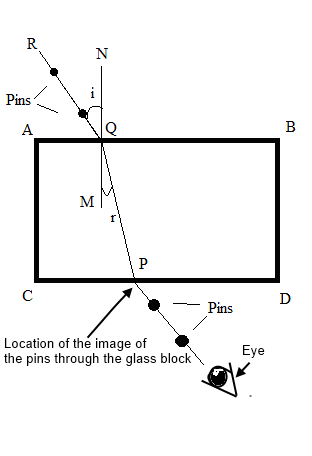
\includegraphics[width=0.49\textwidth]{./img/refractive-index-1.png}
\end{center}

\begin{description*}
%\item[Subtopic:]{}
\item[Materials:]{Glass block, 4 pins, plain paper, ruler, pencil}
%\item[Setup:]{}
\item[Procedure:]{Trace the outline of a glass block ABCD on a piece of paper. Measure an angle of $i=20^\circ$ and stick 2 pins along this line as shown. Draw the normal to the block surface at Q. Look through the other side of the block (CD) horizontally, and place 2 more pins so that they appear in a straight line with the other pins. Remove the pins and connect with a straight line. Connect points Q and P. Measure the value of $r$ as shown in the figure. Repeat for $i=30^\circ$, $40^\circ$, $50^\circ$ and $60^\circ$.}
%\item[Hazards:]{}
\item[Questions:]{Tabulate results for $i$, $r$, $\sin{i}$ and $\sin{r}$. Plot a graph of $\sin{i}$ (vertical) against $\sin{r}$ (horizontal). Find the slope and give its physical meaning.}
%\item[Observations:]{}
\item[Theory:]{Light is refracted through the glass, so when you look through it, the pins appear to lie on a different straight line. The refractive index, $\eta$, can be found by $\eta = \frac{\sin{i}}{\sin{r}}$. Thus, the slope of the graph gives the refractive index of glass, which should be around 1.5.}
%\item[Applications:]{}
%\item[Notes:]{}
\end{description*}

\columnbreak

%\subsection{Critical Angle in Glass}
%\textbf{*NECTA PRACTICAL*}
%
%%\begin{center}
%%\includegraphics[width=0.4\textwidth]{./img/source/.png}
%%\end{center}
%
%\begin{description*}
%%\item[Subtopic:]{}
%%\item[Materials:]{}
%%\item[Setup:]{}
%\item[Procedure:]{Repeat as in \nameref{sub:refr-index-glass}.}
%%\item[Hazards:]{}
%\item[Questions:]{Determine the critical angle of the glass block.}
%%\item[Observations:]{}
%\item[Theory:]{Critical angle, $C$, is found by the relationship $\sin{C} = \frac{1}{\eta}$, where $\eta$ is the refractive index of glass. Use mathematical tables to find the value of $C$. For a glass/air interface, $C$ should be around $42^\circ$.}
%%\item[Applications:]{}
%%\item[Notes:]{}
%\end{description*}

\subsection{Total Internal Reflection}

\begin{center}
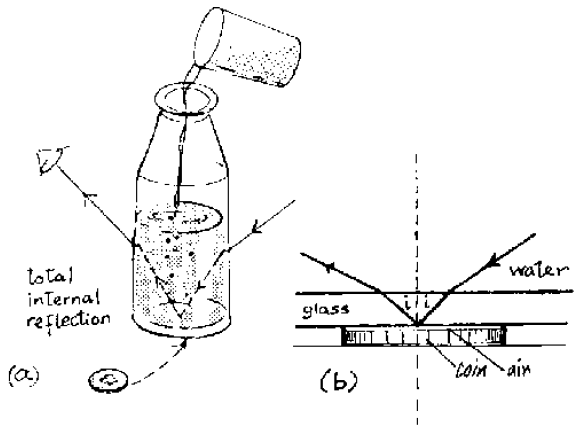
\includegraphics[width=0.35\textwidth]{./img/source/total-int-refl.png}
\end{center}

\begin{description*}
%\item[Subtopic:]{}
\item[Materials:]{Bottle, coin, pitcher of water}
%\item[Setup:]{}
\item[Procedure:]{Place a transparent bottle on a coin and look at the coin from above at an angle from the normal. Pour water into the bottle slowly and notice what happens to the image of the coin.}
%\item[Hazards:]{}
%\item[Questions:]{}
\item[Observations:]{Initially, the coin can be seen. However, there is a level of water at which the coin disappears from sight.}
\item[Theory:]{At the interface between the glass and air above the coin, \emph{total internal reflection} occurs. This only happens at the boundary between an optically denser medium (e.g. glass) and an optically less dense medium (e.g. air) when the angle of incidence in the denser medium is greater than the \emph{critical angle}. The rays coming from the right side hit the bottom of the glass and are totally reflected (no refraction) before meeting your eye. Thus, these strong totally reflected rays of the bottom of the glass completely cover the weaker rays coming from the coin, and so the coin cannot be seen.}
\item[Applications:]{Prisms in binoculars, periscopes}
%\item[Notes:]{}
\end{description*}

%==================================================================================================%

\section*{Refraction by Lenses} \index{Refraction! by lenses}


\subsection{Plastic and Water Lenses}

\begin{center}
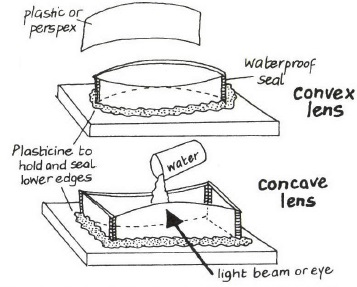
\includegraphics[width=0.45\textwidth]{./img/vso/lenses.jpg}
\end{center}

\begin{description*}
%\item[Subtopic:]{}
\item[Materials:]{Sheets of plastic, candle wax, super glue, board, water}
%\item[Setup:]{}
\item[Procedure:]{Bend the plastic sheets into either a convex or concave shape. Keep them in position by bedding them into candle wax on a board. Seal the edges with wax or super glue. Fill the container with water and it acts as a lens.}
%\item[Hazards:]{}
%\item[Questions:]{}
%\item[Observations:]{}
%\item[Theory:]{}
%\item[Applications:]{}
%\item[Notes:]{}
\end{description*}

\subsection{Focusing an Image Through A Convex Lens}

%\begin{center}
%\includegraphics[width=0.4\textwidth]{./img/source/.png}
%\end{center}

\begin{description*}
%\item[Subtopic:]{}
\item[Materials:]{Convex lens (magnifying glass), white paper or screen, tissue paper, pen, point light source (headlamp, desk lamp, etc.), optional retort stand}
%\item[Setup:]{}
\item[Procedure:]{Cut a piece of tissue paper to fit over the light source. Draw a thick arrow on the tissue paper and tape it over the light source. Shine it directly on a white screen or paper about half a metre away (the distance depends on how strong the light is). Move the magnifying glass/convex lens back and forth between the light and screen until the image of the arrow is focused on the screen. Measure the distances from the lens to the screen and lens to the light source.}
%\item[Hazards:]{}
\item[Questions:]{Calculate the focal length of the lens.}
%\item[Observations:]{}
\item[Theory:]{The lens equation is given as $\frac{1}{f} = \frac{1}{u} + \frac{1}{v}$, where $f$ is the focal length of the lens, $u$ is the distance from the object to the lens, and $v$ is the distance form the focused image to the lens. By focusing the image, we set $u$ and $v$ and can calculate $f$. }
\item[Applications:]{Fry bugs with sunlight}
%\item[Notes:]{}
\end{description*}

\subsection[Magnification Using a Convex Lens]{Magnification Using a \hfill \\ Convex Lens} \index{Magnification}

\begin{center}
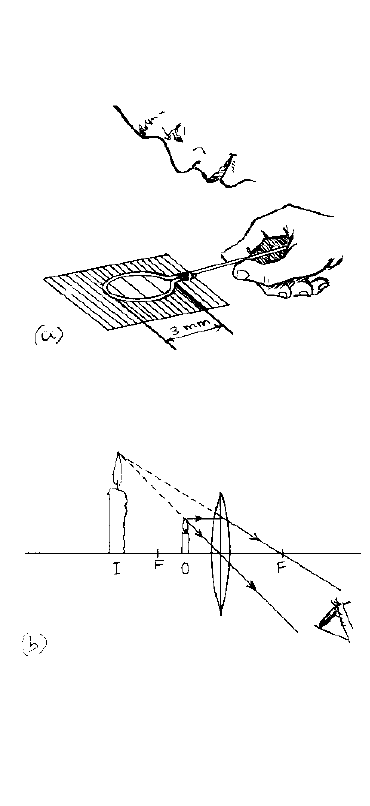
\includegraphics[width=0.45\textwidth]{./img/source/magnification-convex.png}
\end{center}

\begin{description*}
%\item[Subtopic:]{}
\item[Materials:]{Paper clip, water, water bottle}
%\item[Setup:]{}
\item[Procedure:]{Produce a magnifying glass by looping a paper clip wire around the tip of a pen. Dip the loop in water and hold it above letters in a book.}
%\item[Hazards:]{}
%\item[Questions:]{}
\item[Observations:]{The water drop lens acts as a convex lens, magnifying the letter.}
\item[Theory:]{The ray diagram for the convex lens is shown in (b). The image is larger than the object. However, the image is \emph{virtual} because it cannot be obtained on a screen. The object distance $u$ must be less than $f$.}
\item[Applications:]{Magnifying glass, eye lens of compound microscope, telescopes, etc.}
\item[Notes:]{Alternatively, hold a filled water bottle horizontally over the book and look through.}
\end{description*}

\vfill
\columnbreak

%==================================================================================================%

%\section*{Refraction through Prisms}
%
%
%\subsection{Total Internal Reflection in Prisms}
%
%\begin{center}
%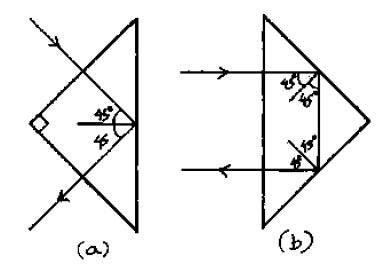
\includegraphics[width=0.4\textwidth]{./img/source/total-int-refl-prism.png}
%\end{center}
%
%\begin{description*}
%%\item[Subtopic:]{}
%%\item[Materials:]{}
%%\item[Setup:]{}
%%\item[Procedure:]{}
%%\item[Hazards:]{}
%%\item[Questions:]{}
%%\item[Observations:]{}
%\item[Theory:]{Total internal reflection occurs when light falls on a glass prism with angles of $45^\circ$, $45^\circ$ and $90^\circ$. This is because a ray falling normally on any face of the prism hits the inside face at $45^\circ$, which is greater than the critical angle of glass/air (about $42^\circ$). In (a) the ray is turned through $90^\circ$ and in (b) through $180^\circ$.}
%\item[Applications:]{See Form I activity on \nameref{sub:i-periscope}, but using 45$^\circ$ prisms in place of mirrors.}
%%\item[Notes:]{}
%\end{description*}

%==================================================================================================%

\section*{Dispersion of White Light}


\subsection{Soap Bubbles}

%\begin{center}
%\includegraphics[width=0.4\textwidth]{./img/vso/soap-bubbles.jpg}
%\end{center}

\begin{description*}
%\item[Subtopic:]{}
\item[Materials:]{Water, soap, water bottle, straw}
%\item[Setup:]{}
\item[Procedure:]{Make a soap solution by mixing water and soap. Place the soap solution near a source of white light or in open sunlight. Immerse the straw into the soap solution and blow into it to form bubbles.}
%\item[Hazards:]{}
%\item[Questions:]{}
\item[Observations:]{Different colours are observed as the sunlight hits the soapy bubbles and undergoes refraction into its component colours.}
\item[Theory:]{Dividing of white light into its colours is called dispersion. This occurs because the light is refracted when passing into the soap and then again when passing back into air.}
%\item[Applications:]{}
%\item[Notes:]{}
\end{description*}

\subsection{Water Prism}

\begin{center}
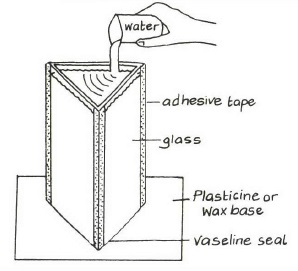
\includegraphics[width=0.45\textwidth]{./img/vso/water-prism.jpg}
\end{center}

\begin{description*}
%\item[Subtopic:]{}
\item[Materials:]{3 small sheets of glass, tape, candle wax, Vaseline}
\item[Setup:]{Stick 3 pieces of glass together with tape. Use Vaseline along the joints to make them watertight. Push the prism into a base of Plasticine or candle wax so it is watertight Fill the prism with water.}
\item[Procedure:]{Shine a beam of light through the prism to view a spectrum of colours.}
%\item[Hazards:]{}
%\item[Questions:]{}
%\item[Observations:]{}
%\item[Theory:]{}
%\item[Applications:]{}
%\item[Notes:]{}
\end{description*}

\columnbreak

\subsection{Mirrors and Water}

\begin{center}
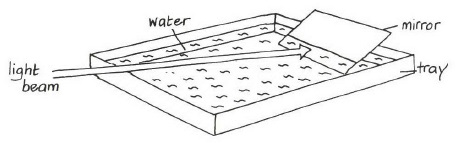
\includegraphics[width=0.49\textwidth]{./img/vso/dispersion-mirror.jpg}
\end{center}

\begin{description*}
%\item[Subtopic:]{}
\item[Materials:]{Plane mirror, tray of water}
%\item[Setup:]{}
\item[Procedure:]{Angle the mirror in the dish of water. Direct a beam of light or sunlight through the water and onto the mirror. Project the light onto a piece of white card or a wall.}
%\item[Hazards:]{}
%\item[Questions:]{}
\item[Observations:]{The spectrum of clours can be seen.}
\item[Theory:]{The refraction of the incident colours on the surface of the water and of the reflected rays makes the water act as a kind of prism.}
%\item[Applications:]{}
%\item[Notes:]{}
\end{description*}

\subsection{Water Hose Rainbow}

\begin{center}
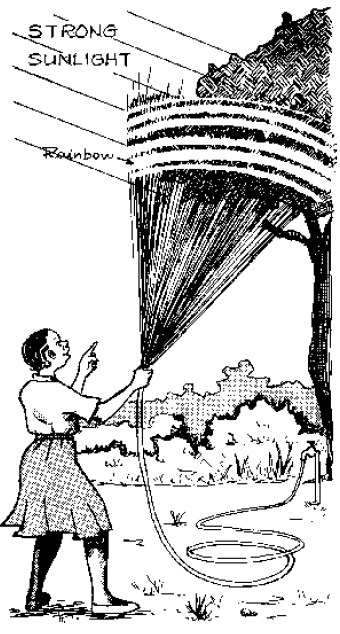
\includegraphics[width=0.35\textwidth]{./img/source/water-hose-rainbow.png}
\end{center}

\begin{description*}
%\item[Subtopic:]{}
%\item[Materials:]{}
%\item[Setup:]{}
\item[Procedure:]{In the early morning or late afternoon on a sunny day spray water from a hose pipe against a dark background of trees with your back towards the sun.}
%\item[Hazards:]{}
%\item[Questions:]{}
\item[Observations:]{The colours of the rainbow can be seen in the spray from the hose.}
\item[Theory:]{The rainbow is the result of the dispersion of light rays striking water droplets.}
%\item[Applications:]{}
%\item[Notes:]{}
\end{description*}

%\columnbreak

%==================================================================================================%

\section*{Colour} \index{Colour|textbf}


\subsection{Colour Wheel}

\begin{center}
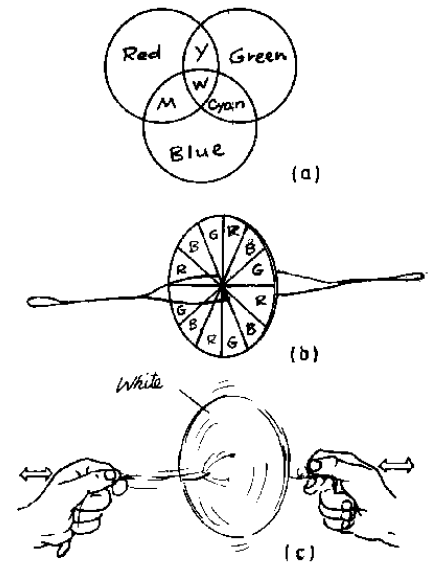
\includegraphics[width=0.45\textwidth]{./img/source/colour-wheel.png}
\end{center}

\begin{description*}
%\item[Subtopic:]{}
\item[Materials:]{White card, string, markers or paint of different colours}
\item[Setup:]{Colour 12 equal sectors of a white card disk with red, green and blue colours arranged in that order as shown. Poke two holes around the centre of the disk and tie a string through them.}
\item[Procedure:]{Swing and pull the string ends with both hands so that the disk spins.}
%\item[Hazards:]{}
%\item[Questions:]{}
\item[Observations:]{The spinning disk appears white.}
\item[Theory:]{Blue, green and red are \emph{primary colours}, meaning they cannot be produced by combining other colours. When combined together, these colours form white light.}
%\item[Applications:]{}
\item[Notes:]{Try making colour wheels using other combinatinos of colours to see how they mix together (e.g. red and orange, blue and yellow, red and green, etc.)}
\end{description*}

\vfill
\columnbreak

\subsection{Batik and Tie Dyeing} \index{Tie-dying}

\begin{center}
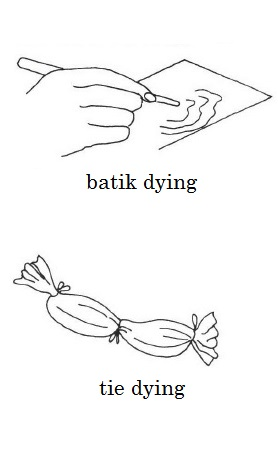
\includegraphics[width=0.4\textwidth]{./img/vso/tie-dyeing.jpg}
\end{center}

\begin{description*}
%\item[Subtopic:]{}
\item[Materials:]{Rosella leaves, coloured flowers, fruits, etc., metal container, candle wax, cloth, fine string}
\item[Setup:]{Crush the flowers or fruit and boil in water for 15 minutes or more. Strain the coloured liquid through a cloth into a bucket.

Experiment with different plants to find new colours. For example:\\
green - spinach or cassava leaves\\
yellow - onion skins\\
brown - tea, coffee, iodine\\
blue - drops of iodine in warm flour solution}
\item[Procedure:]{For batik, draw a design on cloth with molten candle wax. Then place the cloth in the dye. Dye does not affect the waxed areas. After the dye has dried remove the wax by ironing though paper.

In tie dyeing the cloth is pleated and then tied tightly with string. The dye does not penetrate the areas which are tied tightly.}
%\item[Hazards:]{}
%\item[Questions:]{}
%\item[Observations:]{}
%\item[Theory:]{}
%\item[Applications:]{}
%\item[Notes:]{}
\end{description*}

%==================================================================================================%


\end{multicols}

\pagebreak